\documentclass[12pt]{report}
\usepackage[dvipsnames]{xcolor}
\usepackage[utf8]{inputenc}
\usepackage[T1]{fontenc} %font encoding for some characters
\usepackage{csquotes}
\usepackage[french]{babel} %give french translation for most commands
\usepackage{fullpage} %extend document's text width
\usepackage[
style=numeric,
backend=biber,
sortlocale=fr-FR,
language=french,
sorting=none %permet de classer la bibliographie dans l'ordre de citation
]{biblatex}
\addbibresource{bibliographie.bib}
\usepackage{graphicx} %make usage of images simpler
\usepackage{lastpage} %make a usable reference to the lastpage
\usepackage{subfigure} %enable to produce subfigure in figure environment
\usepackage{multicol} %enable multi-columns part easily
\usepackage{lmodern} %some more characters encoding stuff
\usepackage{enumitem} %enable label modification for lists
\usepackage[bottom, perpage]{footmisc} %reset footnote counter each page
\usepackage{tabulary} %able to use tabulary env or set column width in tabular
\usepackage[hidelinks]{hyperref} %enable links creation into the pdf
\usepackage[toc, acronym]{glossaries} %generate glossary with entries used with \gls. Needs to be loaded after hyperref for clickable links
\usepackage[
    %disable,% uncomment this when finished
    french,
    colorinlistoftodos,
    backgroundcolor=blue!40
]{todonotes} %todo list to complete the document
\usepackage{fancyhdr}
\usepackage{float}
\usepackage{lipsum} %generate lorem ipsum
\usepackage{refcount} %used to get refpage as number
\usepackage{xintexpr} %used to have boolean expression
\usepackage{url}
%\usepackage[ddmmyyyy]{datetime} %used for custom \today cmd
\setrefcountdefault{-1} %used to set pagref during compile time

\newcommand{\todoHigh}[1]{\todo[color=Red, inline]{#1}}
\newcommand{\todoCheck}[1]{\todo[color=Orange, inline]{#1}}
\newcommand{\todoOpt}[1]{\todo[color=Cyan, inline]{#1}}

\let\cleardoublepage\clearpage

\setlength{\headsep}{2pt}
\nocite{*} %permet d'écrire toutes les entrées présentes dans la bibliographie sans avoir à les citer
\glsaddall %permet d'écrire toutes les entrées présentes dans le glossaire sans avoir à les citer

\title{Mission en entreprise \\ Mémoire première année}
\author{BROSSARD Florian}
\date{\today}
\newcommand{\schoolyear}{Master ILC 1\iere{} année}
\def\thanks{
    Tuteur universitaire : Stéphane CATELOIN\\
    Maître d'apprentissage : Sabrina MIGNON
}

\newcommand{\pageCount}{
     \xintifboolexpr{ \value{chapter} > 0 && \value{page} <= \getpagerefnumber{Fin}}
        {Page \thepage/\pageref{Fin}} %if part number > 0 AND page number <= pageref{Fin}
        {} %else nothing
}

\newcommand{\footerLeftText}{BROSSARD Florian}
\newcommand{\footerCenterText}{Mission en entreprise - Mémoire première année}
\newcommand{\footerRightText}{\pageCount}

\newcommand{\printAbstract}[4]
{
    \newpage
    \thispagestyle{empty}
    \setlength{\parskip}{-0.5em}
    \vspace*{\fill}
    \vspace{2em}
    \noindent\textbf{\LARGE Résumé}\\
    \p
    #1
    \p
    \textbf{Mots-clés :} #2
    \vspace{1em}
    \hrule
    \vspace{1.5em}
    \noindent\textbf{\LARGE Abstract}\\
    \p
    #3
    \p
    \textbf{Key-words : } #4
    \vspace*{\fill}
}

\newcommand{\fin}
{
    \label{Fin}
    %Fin du document -> affichage bibliographie, glossaire et résumé
    \printglossary
    \printglossary[type=\acronymtype]
    \printbibliography[heading=bibintoc,title={Bibliographie}] %ces paramètres permettent de placer la biblio dans la table des matières
}

\frenchbsetup{StandardLists=true}
\newcolumntype{K}[1]{>{\centering\arraybackslash}p{#1}}
\let\cleardoublepage\clearpage
\setlength{\headsep}{2pt}
\fancypagestyle{plain}{
	\fancyhf{}
	\fancyhead[L]{\ifnum\value{chapter}>0\leftmark\fi}
	\fancyfoot[L]{\footerLeftText}
	\fancyfoot[C]{\footerCenterText}
	\fancyfoot[R]{\footerRightText}
	\setlength{\headheight}{15pt}
}

\fancypagestyle{tocAndLof}{
	\fancyhf{}
	\fancyfoot[L]{\footerLeftText}
	\fancyfoot[C]{\footerCenterText}
	\setlength{\headheight}{15pt}
}

\newcommand{\p}{\paragraph{}}

\newcommand{\reference}[1]{(Voir section \ref{#1} page \pageref{#1})}

\makeglossaries
%\newglossaryentry{SampleGlossRef} 
%{
%    name={Sample Glossary Reference},
%    description={Sample glossary reference description},
%    text={Sample glossary reference} %\gls{SampleGlossRef}
%    plural={Sample Glossary References} %\glspl{SampleGlossRef}
%}

%\newacronym[longplural={Frames per Second}]{fpsLabel}{FPS}{Frame per Second}
%\newacronym{lvm}{LVM}{Logical Volume Manager}

\newacronym{ufr}{UFR}{Unité de Formation de Recherche}

\newacronym{ilc}{ILC}{Ingénierie des Logicielles et des Connaissances}

\newacronym{ihm}{IHM}{Interface Homme-Machine}

\newacronym{es}{ÉS}{Électricité de Strasbourg}

\newglossaryentry{rest}
{
    name={REST},
    description={REST (representational state transfer) est un style d'architecture logicielle, notamment utilisé dans les applications web\cite{wiki:REST}},
    first={REST (representational state transfer)},
    text={Representational state transfer}
}

\newglossaryentry{dmz}
{
    type=\acronymtype,
    name={DMZ},
    description={En informatique, une zone démilitarisée (ou DMZ, de l'anglais demilitarized zone) est un sous-réseau séparé et isolé du réseau local par un pare-feu. Ce sous-réseau contient les machines étant susceptibles d'être accédées depuis Internet.\cite{wiki:DMZ}},
    text={DMZ}
}

\newglossaryentry{tma}
{
    type=\acronymtype,
    name={TMA},
    description={La Tierce Maintenance Applicative consiste à externaliser la maintenance de toutes ou d'une partie des applications d'une entreprise auprès d'un prestataire},
    first={tierce maintenance applicative (TMA)},
    text={TMA}
}

\newglossaryentry{gwt}
{
    name={GWT},
    description={Framework permettant de créer et maintenir des applications web dynamiques mettant en œuvre JavaScript, en utilisant le langage et les outils Java},
    first={GWT (Google Web ToolKit)},
    text={GWT}
}

\newglossaryentry{gxt}
{
    name={GXT},
    description={Framework permettant de créer des applications web riches en utilisant GWT},
    first={GXT},
    text={GXT}
}

\newglossaryentry{vm}
{
    name={Machine virtuelle},
    description={Une machine virtuelle est une simulation d'un appareil informatique créée par un logiciel},
    first={machines virtuelles},
    text={Machine virtuelle}
}

\newglossaryentry{sts}
{
    type=\acronymtype,
    name={STS},
    description={Sprinsource Tool Suite est une distribution du logiciel \gls{eclipse} facilitant le développement d'application Web JAVA utilisant le framework \gls{spring}},
    text={STS}
}

\newglossaryentry{eclipse}
{
    name={Eclipse},
    description={Eclipse est un \gls{ide} libre et extensible pour le language JAVA},
    text={Eclipse}
}

\newglossaryentry{ide}
{
    type=\acronymtype,
    name={IDE},
    description={. Un IDE (pour Integrated Development Environment) rassemble un enemble d'outils permettant d'augmenter la productivité des développeurs en un seul logiciel},
    text={IDE}
}

\newglossaryentry{spring}
{
    name={Spring},
    description={Le framework Spring permet de construire et de définir l'infrastructure d'une application JAVA},
    text={Spring}
}

\newglossaryentry{maven}
{
    name={Maven},
    description={Outil de gestion et d'automatisation de production des projets logiciels Java},
    text={Maven}
}

\newglossaryentry{svn}
{
    name={SVN},
    description={Subversion (en abrégé svn) est un logiciel de gestion de versions\cite{wiki:svn}},
    text={SVN}
}


\newglossaryentry{webservice}
{
    name={Webservice},
    description={Logiciel sans interface permettant la communication et l'échange de données entre applications et systèmes hétérogènes},
    text={Webservice}
}

\newglossaryentry{rpc}
{
    type=\acronymtype,
    name={RPC},
    description={En informatique, Remote Procedure Call (RPC) désigne un protocole réseau permettant de faire appels à des procédures sur un ordinateur distants à l'aide d'un serveur d'applications},
    text={RPC}
}

\newglossaryentry{dao}
{
    type=\acronymtype,
    name={DAO},
    description={Un DAO (Data Access Object) est un patron de conception permettant d'ajouter une couche d'abstraction concernant le stockage de données},
    text={DAO}
}

\newglossaryentry{dto}
{
    type=\acronymtype,
    name={DTO},
    description={Un objet de transfert de données (Data Transfer Object en anglais) est un patron de conception utilisé dans les architectures logicielles objet. Il permet de simplifier la transmission de donner entre les différentes couches d'une application},
    text={DTO}
}

\newglossaryentry{ajax}
{
    type=\acronymtype,
    name={AJAX},
    description={L'architecture AJAX, acronyme d'Asynchronous JavaScript and XML, permet de créer des applications web dynamique et interactive\cite{wiki:AJAX}. Cela permet entre autre de modifer une partie de la page sans devoir la recharger entièrement},
    text={AJAX}
}

\newglossaryentry{sgbd}
{
    type=\acronymtype,
    name={SGBD},
    description={En informatique, un système de gestion de base de données (abr. SGBD) est un logiciel système destiné à stocker et à partager des informations dans une base de données\cite{wiki:SGBD}},
    first = {Système de Gestion de Base de Données (SGBD)},
    text={SGBD}
}

\newglossaryentry{hibernate}
{
    name={Hibernate},
    description={Hibernate est un framework open source gérant la persistance des objets en base de données relationnelle\cite{wiki:hibernate}},
    text={Hibernate}
}

% Début du document

\begin{document}
    
    \makeatletter
    \begin{titlepage}
		\enlargethispage{2cm}
		\begin{center}
			
\includegraphics[width = 50mm]{img/unistra.jpg} \hfill
			
\includegraphics[width = 70mm]{img/logoUFRMath.png} 
		\end{center}
		
		\begin{center}
			\vspace*{3cm}
			\LARGE{\@author\\}
			\large{\schoolyear \\ \@date}
			\vspace*{1cm}
			\hrule
			\vspace*{0.5em}
			\textsc{\LARGE{ \@title }}
			\vspace*{1em}
			\hrule
		\end{center}
		\begin{center}
			\vspace{1.5cm}
			
\includegraphics[width = 60mm]{img/atos.png} \hfill
			
\includegraphics[height = 25mm]{img/es.jpg} \\
			\vspace{2cm}
			\thanks
		\end{center}
	\end{titlepage}
    \makeatother
    
    \listoftodos\thispagestyle{empty}
    \newpage
    
    %Page remerciements
    \thispagestyle{empty}
    \vspace*{\fill}
    \begin{center}
    	\Large{\textbf{Remerciements}}
    \end{center}
    \setlength{\parskip}{1em}
    ~\\
    \indent Je tiens à remercier l’ensemble des membres du personnel travaillant au sein des société ES et Atos pour leur gentillesse, leur accueil et leur disponibilité.
    
    Je remercie Mme. MIGNON Sabrina, chef de projet chez Atos et mon maître d'apprentissage, pour le temps qu'elle m'a accordé afin de me former et de m'aider.
    
    Je tiens également à remercier M. CATELOIN Stéphane, mon tuteur à l’université, pour la rapidité et la clarté avec lesquelles il a su répondre à mes questions pendant mon apprentissage.
    \vspace*{\fill}
    
    \setlength{\parskip}{0em}
    \pagestyle{tocAndLof}
    \tableofcontents
    \listoffigures
    \clearpage
    
    \pagestyle{plain}
    \setlength{\parskip}{1em}
    \setcounter{page}{1}
    
    \chapter{Contexte}
    \todoHigh{Désactiver les todos une fois le document terminé}
    Lors des deux ans de Master \acrfull{ilc}, les étudiants doivent effectuer une partie de leur scolarité en apprentissage au sein d'une société. Le temps de travail est partagé entre le temps en entreprise et le temps à l'université, durant la première année, à hauteur de 2 jours à l'université et 3 jours en entreprise.
    
    J'ai eu la chance de pouvoir intégrer la société Atos en tant qu'apprenti en travaillant au sein de l'équipe Atos localisée dans les bureaux d'un de leur client : \acrfull{es}.
    
    Dans ce mémoire, vous trouverez le travail effectué en entreprise durant la première année d'alternance. Dans un premier temps nous présenterons les groupe Atos et \acrshort{es}, avec une description des activités d'Atos chez \acrshort{es}. Suite à cela, une partie du mémoire sera consacrée à l'environnement de travail, puis aux différents projets abordés et futurs. Nous conclurons par un bilan général concernant les impressions dans le cadre professionnel et personnel.
	
	\newpage
	
	\section{Le groupe Atos}
	Atos est un leader international de la transformation digitale\footnote{Désigne le processus au cours duquel une entreprise intègre les technologies disponibles pour ses activités.}, du conseil et des services informatiques.
	Le groupe est implantée dans 73 pays, compte plus de 100 000 collaborateurs et réalise plus de 13 Milliards d'euros de chiffres d'affaires annuel.
	
	\begin{figure}[ht]
	    \centering
	    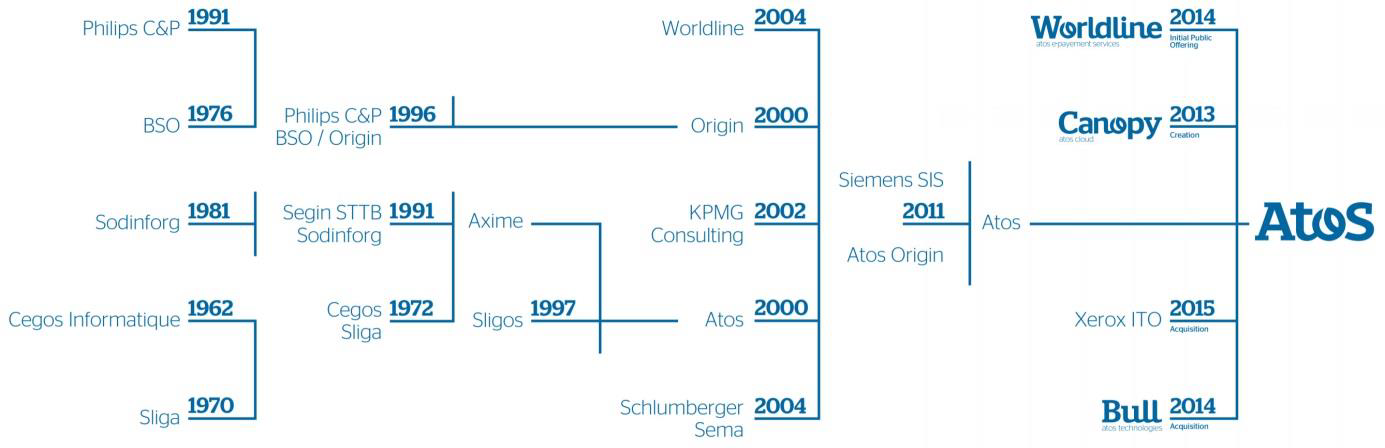
\includegraphics[width=0.99\textwidth]{img/Atos_acquisition_filiale.png}
	    \caption{Acquisitions et filiales d'Atos\cite{TweetAtosAcquisition}}
	    \label{fig:atos_acquisition}
	\end{figure}
	
	Atos étend ses activités par le biais d'acquisitions succéssives, parmis lesquelles on retrouve :\vspace{-1.5em}
	\begin{itemize}[itemsep=-0.5em]
	    \item L'infogérence et le conseil
	    \item Le cloud
	    \item Les services de e-paiement avec sa filiale Wordline
	    \item La cybersécurité
	    \item La défense et les sytèmes critiques
	\end{itemize}
	
	Atos est également le partenaire de grands groupes tel que Microsoft, Cisco et Oracle afin de pouvoir fournir au client des solutions innovantes.
	
	\newpage
	
	\section{Le groupe ÉS}
	Le groupe \acrshort{es} (\acrlong{es}), énergéticien régional multi-énergies en Alsace depuis plus de 100 ans et filiale d'EDF, fait partie des grands acteurs du secteur énergétique français. Le groupe, organisé autour de trois grandes activités, est composé :
	\begin{itemize}
	    \item d’un opérateur et gestionnaire de réseaux : Strasbourg Électricité Réseaux
	    \item d'une filiale commerciale : ÉS Énergies Strasbourg
	    \item de deux filiales spécialisées dans les services énergétiques et les énergies renouvelables : ÉS Services Énergétiques et ÉS Géothermie
	\end{itemize}
	
	\begin{figure}[ht]
	    \centering
	    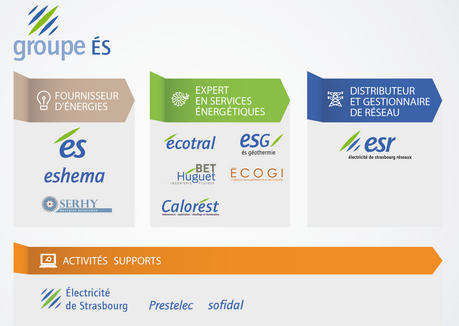
\includegraphics[width=0.9\textwidth]{img/orga_ES.png}
	    \caption{Organisation du groupe \acrshort{es}\cite{OrganisationES}}
	    \label{fig:orga_es}
	\end{figure}
	
	\newpage
	
	\section{Les activités d'Atos chez ÉS}
	\label{atos_es}
	Dans le cadre du contrat de \gls{tma} entre Atos (anciennement Bull) et \acrshort{es}, plusieurs équipes d'Atos sont présentent au centre opérationnel de Mundolsheim du groupe \acrshort{es}.
    Elles sont organisés en deux lots:
    \begin{itemize}
        \item Le lot 1, dont je fais partie, est chargé de la maintenance applicative et évolutive JAVA,  ainsi que des projets complémentaires.
        \item Le lot 2 est l’équipe décisionnelle.
    \end{itemize} 
    
    \subsection{Composition de l'équipe TMA JAVA}
    Le directeur de projet des équipes Atos est Jean-Pierre FONNE.
    
    L'équipe \gls{tma} JAVA comprend 8 personnes:\vspace{-1em}
    \begin{itemize}[itemsep=-0.5em]
        \item MIGNON Sabrina, référant projet
        \item RICHARD Alexandre, référant TMA
        \item QUERE Alexandre
        \item TERREAUX Mathias
        \item MONTESANTOS Alexis
        \item GRILL Stéphane
        \item MARLIER David
        \item TURIN Gary
        \item BROSSARD Florian (Apprenti)
    \end{itemize}
    On distingue deux activités au sein de cette équipe :\vspace{-1em}
    \begin{description}
        \item[La \gls{tma} :] Consiste en la réalisation de correctifs en cas d'anomalies déclarées, et/ou d'évolutions mineures suite à une demande ou à l'évolution d'un logiciel.
        \item[Les projets :] Consiste en la création de nouvelles applications suivant le besoin du client.
    \end{description}
    
    Les utilisateurs déclarent les incidents via l'application PICTO. Ces demandes sont ensuite transférées au responsable de domaine fonctionnel qui valide l’incident et missionne la \gls{tma} pour le résoudre, suivant leurs ordre de priorité.
    
    \chapter{Environnements de travail}
    
    \section{Intégration à l'équipe}
    Durant la première semaine, j'ai suivi une formation concernant l'architecture \acrshort{rest} ainsi que sur l'environnement de développement JAVA utilisé par l'équipe. Nous utilisons entre autre les framework \gls{gwt} et \gls{gxt}.
    
    Ma charge de travail est répartie majoritairement sur du temps de projet.
    
    Durant le travail que j'ai effectué sur le projet pApps \reference{papps}, il m'à été demandé de créer une application ayant une interface différente des applications internes auxquelles les employés sont habitués. Pour cela, j'ai du rechercher comment modifier l'aspect des composants graphiques du framework \gls{gxt}. Ceci m'à donné l'occasion de faire une présentation à toutes l'équipe de la TMA JAVA et certains membres d'ÉS, permettant ainsi de partager l'information afin de gagner du temps à l'avenir.
    
    \newpage
    
    \section{Technologies utilisés}
    
    \subsection{Développement JAVA}
    L'équipe \gls{tma} JAVA a à sa disposition plusieurs \gls{vm}. Chaque développeur dispose donc du même environnement de travail. Suivant la version de \gls{gxt} utilisée, nous développons sur \gls{sts} pour \gls{gxt} 2 et sous \gls{eclipse} Mars pour \gls{gxt} 3.
    
    Le navigateur cible des applications développées par l'équipe est Internet Explorer.
    
    Pour chaque projet nous utilisons un archetype \gls{maven} prédéfinis (application web ou \gls{webservice}), chaque application est séparées en plusieurs couches :\vspace{-1em}
    \begin{itemize}[itemsep=0em]
        \item Couche DAO : Gère l'accès aux bases de données et les requêtes.
        \item Couche Service : Effectue les traitements métiers, fait appel aux \glspl{webservice}
        \item Couche Server (application seulement) : Couche d'abstraction afin de faire appels au méthodes de la couche service.
        \item Couche RPC (application seulement) : Contient les interfaces synchrones et asynchrones des services de \gls{gwt}, les \gls{dto} et les classes utilitaires. Cette couche permet de faire le lien entre le client et le serveur.
        \item Couche RS (\gls{webservice} seulement) : Point d'entrée des méthodes de la couche service. Fait appels aux méthodes de la couche service.
        \item Couche Webapp (application seulement): Gère l'interface graphique, l'authentification et contient les ressources statiques de l'application (images, feuilles CSS, ...)
        \item Couche Interface (\gls{webservice} seulement) : Contient l'interface des services exposés par le \gls{webservice}.
    \end{itemize}\vspace{-0.5em}
    
    Nous utilisons également \gls{maven} pour gérer les dépendences des projets.\vspace{-0.5em}
    \newpage    
    \subsection{Intégration continue et qualité de code}
    
    Afin d'améliorer la productivité et l'éfficacité des développeurs, plusieurs outils sont mis à notre disposition :
    \begin{itemize}[itemsep=0em]
        \item \gls{svn} : notre logiciel de gestion de versions
        \item Jenkins : logiciel open source d'intégration continue. Il permet de déployer rapidement et simplement les différents projets, mais peut également lancer des tâches définies, notamment afin de lancer un scan SonarQube via la même interface que pour les déploiements.
        \item SonarQube: SonarQube est un logiciel libre permettant de mesurer la qualité du code source à l'aide de nombreuses règles définies. SonarQube lance régulièrement une analyse des différents projets afin d'afficher la qualité générale du code, proposant ensuite des solutions aux bugs potentiels (pointeur null par exemple) et mauvaises pratiques et des améliorations concernant la lisibilité du code, notamment via les règles de codage (indentation, conventions de nommage, etc...).
    \end{itemize}
    
    Ces logiciels nous permettent d'une part de travailler en groupe, d'autre part d'améliorer la qualité des projets en général, les rendant plus facilement maintenable, mais aussi et surtout ils nous permettent d'être réactifs, c'est-à-dire de pouvoir traiter et corriger plus de problèmes avant que les utilisateurs n'y soient confrontés.
    
    \subsection{GWT / GXT}
    Pour développer l'\acrfull{ihm} des applications web, nous utilisons les frameworks \gls{gwt} et \gls{gxt}. Ceci nous permet d'utiliser une langage objet de haut niveau (en l'occurence JAVA) ainsi que les outils disponibles pour ce language (débuggers, bibliothèques). En resumé, ces deux framework nous permettent de développer nos applications de la même manière qu'une application JAVA Swing\footnote{Bibliothèque graphique JAVA}, à ceci près que l'on utilise les widgets de GWT et de GXT pour former l'interface. Ensuite le compilateur de GWT transforme le code JAVA en code Javascript tout en gérant la compression des ressources (images, texte, etc...), la gestion du cache et des appels \gls{ajax}.
    
    \newpage
    
    \subsection{Base de données et persistance des données}
    Nous utilisons le \gls{sgbd} Oracle pour stocker les données persistantes des applications. La gestion de la sauvegarde, suppression, mise à jour, et même le filtrage des différents objets sont effectués à l'aide du framework \gls{hibernate}. Pour ce faire chaque objet persistant se voit lié à une entité et un \gls{dao} dont tous les champs sont mappés\footnote{Signifie ici faire correspondre.} à une colonne d'une table à l'aide d'\gls{hibernate}. Cette table servira donc à stocker chaque objet d'une même classe JAVA.
    
    Nous avons également à notre disposition deux logiciels afin de faciliter la gestion et la modification des base de données :
    \begin{description}
        \item[PowerAMC: ]Logiciel permettant de modèliser graphiquement une base de données. Nous pouvons ainsi facilement créer des relations entre plusieurs tables, des contraintes, des vues, etc..., à l'image des logiciels utilisant le glisser-déposer tel que PowerPoint. PowerAMC génère ensuite un script SQL à éxécuter sur la base de donnée afin d'y ajouter, modifier ou supprimer les différentes table. Parmis ses autres fonctions, les plus intéressantes sont la \gls{retroingenierie}, permettant de générer un schéma à partir de la base de donnée, et la génération d'un script SQL modifiant la base de données, permettant de ne modifier que ce qui est nécessaire, et de garder les données présentes dans la mesure du possible.
        \item[SQL Developper: ]Outil graphique permettant de parcourir et d'interroger de multiple bases de données. Il permet entre autre d'éxécuter des requêtes SQL directement sur les bases de données, de rechercher et filtrer les différentes tables et les champs de ces tables, ainsi que leurs données. Son éditeur de requête est doté d'un vérificateur de syntaxe affichant les erreurs ainsi que des proposition de corrections pour celles-ci. Ce logiciels possèdent d'autres fonctions utiles tel que le rollback, permettant d'annuler des modifications en base, ou encore l'importation et exportation de données, utile pour utiliser un jeu de données spécifique pour les tests unitaires d'une application.
    \end{description}
    
    \chapter{Projets}
    
    \section{Histo-versions}
    L'application histo-versions a été le premier projet qui m'a été confié. Le but de cette application est d'afficher l'historique des déploiements des différentes applications pour chaque environnement. Afin d'éviter tout malentendu, sauf mention contraire, nous parlerons de création et de suppression d'application au sein d'histo-versions en parlant de l'ajout ou la suppression de lignes dans la table listant les applications, utilisée par histo-versions.
    
    \begin{figure}[ht]
        \centering
        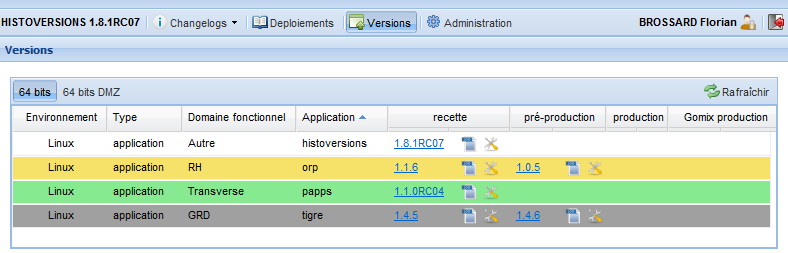
\includegraphics[width=0.99\textwidth]{img/HV_Panel_versions.png}
        \caption{Panneau "Versions" d'histo-versions}
        \label{fig:histoversions_versions}
    \end{figure}
    
    \newpage
    
    \subsection{Les environnements}
    Voici le cheminement du déploiement d'une nouvelle version d'une application:\vspace{-1em}
    \begin{enumerate}
        \item Lorsque le développement d'une évolution ou d'un correctif est terminé, une nouvelle version est déployée sur l'environnement dit de \textbf{recette}. Notre équipe a pleinement accès à cet environnement afin de déployer une nouvelle version.
        \item Suite à la confirmation du chef de projet et du responsable de domaine fonctionnel l'application peut, suite à des tests, être déployée sur l'environnement dit de \textbf{production}. C'est l'environnement qu'utilisent les utilisateurs.
        \item Éventuellement, une application peut être placée dans une environnement dit de \textbf{pré-production}, avant d'être placée sur l'environnement de \textbf{production}, si cela est nécessaire.
    \end{enumerate}
    
    \subsection{Fonctionnalités attendues}
    Voici une liste des fonctionnalités de l'application:\vspace{-1em}
    \begin{itemize}
        \item Afficher la liste des applications avec le numéro de la version déployée pour chaque environnement (\textbf{recette, pré-production, production} et leur équivalent \textbf{\gls{dmz}})
        \item Afficher la liste des changelogs\footnote{Un changelog, ou journal des modifications, est une liste des modifications\cite{wiki:changelog}.} pour chaque application
        \item Afficher la liste de tous les déploiements de chaque application dans chaque environnement
        \item Pouvoir effectuer plusieurs opérations dont la sélection des applications à afficher, l'ajout/suppression de ces applications et des changelogs dans histoversions et le filtrage des applications (par nom, version, environnements, etc...)
    \end{itemize}
    
    
    \subsection{Premiers travaux effectués}
    
    Durant les premiers mois de mon alternance, j'ai débuté une amélioration de la qualité de code, évaluée par le logiciel SonarQube, me permettant ainsi de me familiariser avec plusieurs outils, tel que \gls{svn} et Jenkins, ainsi qu'avec le framework \gls{gxt} 2.Dans le même temps, cela m'as permis de comprendre le fonctionnement de ce projet, facilitant grandement les futures modifications.
    
    Outre les modifications de l'interface et les corrections de bugs, la première tâche que j'ai effectuée à été de rendre périodique l'ajout automatique des déploiements dans la base de donnée. Cet ajout est réalisé à l'aide d'un batch\footnote{En informatique, un traitement par lots (batch processing en anglais) est un enchaînement automatique d'une suite de commandes (processus) sur un ordinateur sans intervention d'un opérateur\cite{wiki:batch}} JAVA. Pour ce faire j'ai dû modifier ce batch afin de pouvoir l'utiliser en tant que tâche, au lieu d'être utilisé en tant que webservice, accessible depuis un lien web.
    
    La première solution afin de pouvoir gérer la plannification à été d'utiliser une fonctionnalité de Spring permettant d'instancier un objet, et de lancer une des méthodes de cet objet à un intervalle donnée. Afin de permettre la modification de cet intervalle, plusieurs variables ont été ajoutées dans le fichier de configuration d'Histoversions.
    
    \subsection{Modifications du batch JAVA}

    La premier changement majeure à été de déplacer l'écran d'administration dans une autre application sur laquelle j'ai travaillé : pApps \reference{portageEcranApplications}.
    
    D'autre part, le batch JAVA qui était en place à nécessité plusieurs modifications suite à plusieurs demandes de fonctionnalités.
    
    La première fonctionnalité à ajoutée était de créer une servlet, appelée depuis une URL, renvoyant la date du dernier déploiement enregistré pour une application et un environnement donné en paramètre. Avec cela, la servlet devait pouvoir mettre à jour les données de la tables concernant l'application et l'environnement spécifiés avant de renvoyer le résultat et, renvoyer un code HTTP et un message d'erreur adéquat dans le cas ou l'application ou l'environnement ne seraient pas trouvés. Cette fonctionnalité à nécessité de modifier le batch de tel sorte que l'on puisse spécifier sur quel environnement et quel applications effectuer le traitement, dans le but de ne mettre à jour que l'application dans l'environnement concerné, et donc de gagner en temps de réponse et de réduire le coup de l'appel à la servlet.
    
    Suite au développement de cette serlvet, une nouvelle spécification à été formulée : supprimer les applications qui ne sont trouvées sur auncun des serveur connus en base. Cette spécification répond au cas où une application serait supprimée du serveur, auquel cas il est nécessaire de faire suivre l'information aux différentes tables d'Histoversions.
    
    \newpage
    
    Après cette modification, la solution ayant été choisie concernant l'appel périodique au batch JAVA à fait apparaitre une erreur de conception : 
    \begin{itemize}[itemsep=1pt, topsep=1pt]
        \item Les base de données sont sauvegardées chaque semaine le week-end, entrainant l'impossibilité de les interroger durant cette opération
        \item Le batch se lance toute les heures chaque jours
        \item Ce même batch supprime les applications qui ne sont pas trouvées, or, la base ne répond pas pendant sa sauvegarde
        \item De plus, dans le cas d'un appel à la serlvet décrite plus haut, si le serveur n'existe pas, ou plus, mais que l'application existe, cette dernière seras tout de même supprimée de la base
    \end{itemize}
    
    Afin de pallier à cette erreur de conception, une autre fonctionnalité à été adopté à la place de l'utilisation d'un intervalle : l'utilisation d'expression CRON. Ce type d'expression permet de spécifier non seulement un intervalle à la seconde près, mais aussi les jours de la semaine, ou du mois auquel on souhaite lancer une tâche.
    
    Pour finir, une légère modification à permis d'éviter de supprimer les applications dans le cas ou le batch est lancé à partir de la servlet.
    
    \section{pApps}
    \label{papps}
    Dans le cadre de mon apprentissage et de ma formation, le projet pApps m'a été confié.
    
    Le projet pApps (pour portail applications) est né d'un besoin de proposer aux utilisateurs un portail d'accès centralisé aux applications. Ce projet remplacera donc l'actuel accès aux applications par leurs adresses.
    
    \newpage
    
    \subsection{Analyse de la demande}
    \subsubsection{Fonctionnalités}
    Voici la liste des fonctionnalités spécifiées dans la documentation fonctionnelle :\vspace{-1em}
    \begin{itemize}[itemsep=1pt]
        \item Afficher une liste des applications
        \item N'afficher que les applications auxquelles l'utilisateur a accès
        \item Afficher, si possible, une icône représentant l'application
        \item Afficher l'environnement des applications
        \item Déplacer la gestion des applications d'Histoversions vers pApps
        \item Modifier les styles de GXT pour créer une interface plus convivial et agréable, différentes des autres
    \end{itemize}
    
    Afin de répondre à ces attentes, nous pouvons utiliser un webservice deja existant, nommé LDAP, permettant de lister les applications auxquelles l'utilisateur a accès. Les icônes des applications peuvent être recherchées sur le serveur, en supposant que l'on respecte un certain formattage du nom des fichiers. Dans le cas où une image n'est pas trouvée, on peut la remplacer par une image par défaut, le logo du groupe \acrshort{es} par exemple.
    
    \subsubsection{Gestion des applications}
    
    Cette fonctionnalité montre la proximité entre les applications pApps et Histoversions. En effet, l'applications Histoversions utilise plusieurs table contenant les informations sur les applications, leurs versions et leurs déploiements. La table contenant les applications étant alimentée par un batch Informatica\footnote{Technologie utilisée par le lot 1 \reference{atos_es} permettant dans ce cas de récupérer des informations à partir des fichiers de projet Maven}, nous pouvons l'utiliser pour le projet pApps, permettant ainsi d'éviter la duplication de données. Il est néanmoins nécessaire de pouvoir saisir et modifer manuellement les applications via un écran car il n'est pas possible de lier directement les applications présentes dans cette table, aux applications récupéré par le webservice LDAP.
    
    \label{portageEcranApplications}
    Cette fonctionnalité a nécessitée de déplacer la gestion des applications d'Histoversions dans pApps. La difficulté de ce travail a été de porter une grille du framework GXT 2 vers GXT 3. Ce problème ayant déjà été soulevé dans d'autre application, deux solutions ont été envisagées : le portage manuelle et l'automatisation.
    
    Dans le cadre de l'évolution de plusieurs autres applications, des recherches et essais avaient déjà été effectués par certains de mes collègues afin d'automatiser le processus de migration d'une version à l'autre de GXT. Ceux-ci n'ayant pas totalement abouti, notamment à cause des différences majeures entre ces deux versions, il à été nécessaire de faire la migration manuellement, posant quelques difficultés étant donné qu'un même objet ou méthode peut avoir un comportement différent, voire même ne pas avoir d'équivalent.
    
    \subsubsection{Interface}
    Concernant l'affichage des environnements des applications, nous avons imaginé deux solutions:\vspace{-1em}
    \begin{itemize}
        \item Plusieurs onglets regroupant chacun les applications d'un seul environnement, avec le nom de l'environnement en guise de label pour l'onglet
        \item Si l'on considère que chaque application est représentée par une tuile, on mettre une couleur de fond et un motif à cette tuile pour indiquer l'environnement.
    \end{itemize}
    On peut également combiner ces deux solutions en mettant par exemple une légende à un endroit visible de la fenêtre, indiquant pour chaque couleur le nom de l'environnement. Chaque élément de cette légende étant cliquable, on peut appliquer un filtrage sur les environnements.
    
    C'est d'ailleurs cette solution que j'ai proposée en premier lieu:
    
    \begin{figure}[ht]
        \centering
        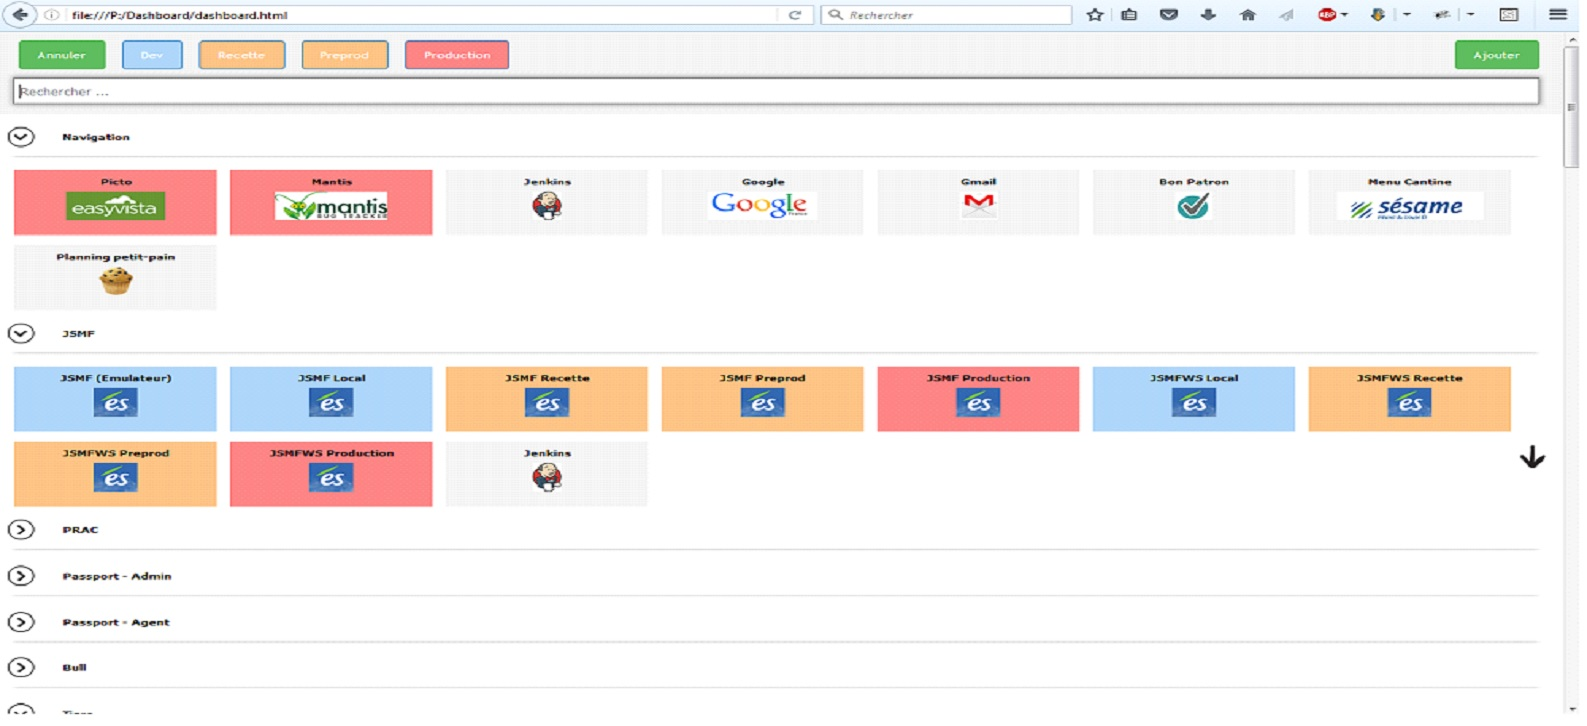
\includegraphics[width=0.8\textwidth]{img/interface_proposition_sfd.jpg}
        \caption{Interface proposée pour pApps}
        \label{fig:papps_interface_proposée}
    \end{figure}
    
    \newpage
    
    Cette première solution a été partiellement retenue :
    \begin{itemize}[itemsep=1pt]
        \item Un seul environnement est affiché à l'écran
        \item Sélection de l'environnement affiché à l'aide de boutons (fonctionnement similaire à des onglets)
        \item Applications affichées sous forme de tuiles avec une icône par défaut
        \item Choix de couleurs neutre (blanc largement majoritaire)
        \item Système d'accordéons permettant de classer les applications par domaine fonctionnel
        \item Barre de recherche
    \end{itemize}
    
    Voici un aperçu de l'interface actuelle :
    
    \begin{figure}[ht]
        \centering
        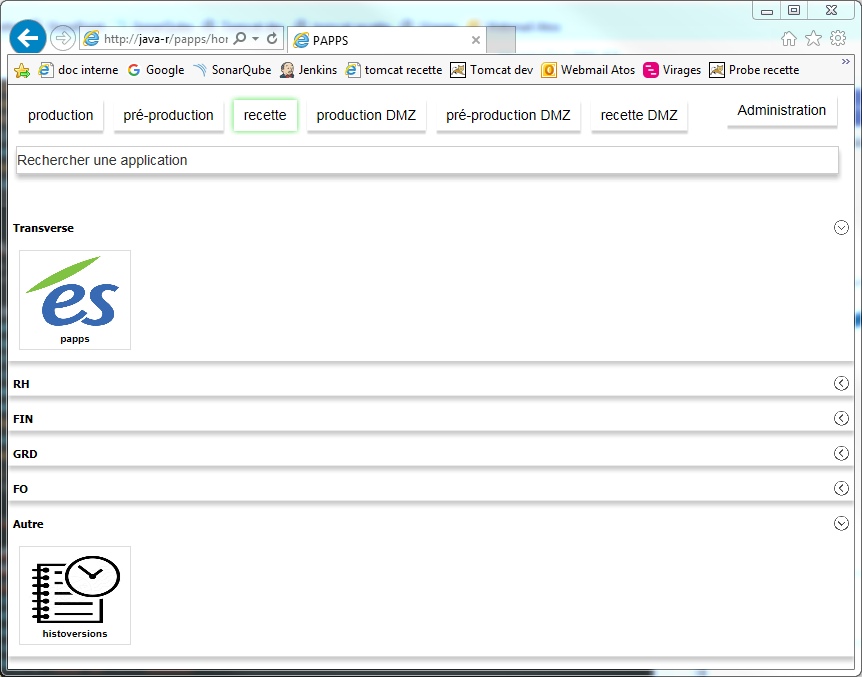
\includegraphics[width=0.99\textwidth]{img/interface_actuelle_papps.png}
        \caption{Interface actuelle de pApps}
        \label{fig:papps_interface_actuelle}
    \end{figure}
    
    \subsection{Organisation du projet}
    
    Afin de prendre en compte au plus tôt les nouvelles demandes, les éventuels problèmes de conception, ainsi que d'assurer le suivi du développement de l'application, nous avons adopté un modèle orienté méthode agile\footnote{Les méthodes agiles se veulent plus pragmatiques que les méthodes traditionnelles, impliquent au maximum le demandeur (client). Elles reposent sur un cycle de développement itératif, incrémental et adaptatif\cite{wiki:agile}.} au lieu du modèle du cycle en V\footnote{Le modèle du cycle en V (en comparaison avec les méthodes dites agiles) est un modèle conceptuel de gestion de projet imaginé\cite{wiki:cycleV}.} habituel. Ceci implique l'organisation de réunion régulière avec le responsable de projet du groupe \acrshort{es}, afin de discuter et valider chaque partie de l'application une par une.
    
    Cette méthode de travail permet notamment de gagner du temps, en évitant des erreurs de conception coûteuses en terme de temps et de modification, ou encore d'ajouter ou préciser certaines demandes et fonctionnalités. Tout cela permet de planifier plus facilement le développement d'une application.
    
    \subsection{Situation actuelle du projet}
    
    Une des tâche majeure a été de récupérer les droits applicatifs de l'utilisateur actuel afin de n'afficher que les applications auquel il est autorisé d'accéder. Pour ce faire, un webservice dédié existant à été utilisé.
    
    Suite à la création du portail, et au portage de l'administration des applications, une fonctionnalité nécessaire au bon fonctionnement est apparue : le mode de compatibilité.
    
    Le mode de compatibilité est en fait un raccourcis pour indiquer qu'une application doit être accéder depuis une URL différente suivant la version de GXT utilisée. Si l'application utilise GXT 2, aucun changement n'est nécessaire. En revanche, si elle utilise GXT 3, on doit modifier l'URL d'accès.
    
    Prenons un exemple concret :
    \begin{itemize}[itemsep=1pt, topsep=1pt]
        \item L'application Histoversions utilise GXT 2
        \item L'application pApps utilise GXT 3
        \item Toute deux sont sur un serveur de \textbf{recette}, dont l'URL d'accès pour GXT 2 est vm-tomcat64-r
        \item Le serveur de recette utilisé habituellement pour les application GXT 2 force un mode de compatibilité concernant la version de JavaScript utilisée, contrairement à GXT 3.
    \end{itemize}
    
    Connaissant ces différents points, une modification s'est avérée nécessaire. Cependant, étant donnée la nature du problème, et après analyse de pApps et d'Histoversions qui partagent les même tables, seules de légères modifications ont été suffisantes pour le résoudre :
    \begin{itemize}[itemsep=1pt]
        \item Ajout d'une colonne indiquant si l'application nécessite le mode de compatibilité, dans la base de donnée et dans l'interface
        \item Ajout d'une colonne indiquant le lien utilisé par le mode de compatibilité dans la table contenant les environnements
        \item Modification des deux vues utilisées pour lister les environnements et les applications pour remplacer le lien du serveur, si le mode de compatibilité est utilisé
    \end{itemize}
    
    Que l'URL soit celui du mode de compatibilité ou non, l'accès au applications reste le même, ce qui explique le peu de modifications nécessaire dans le code source.
    
    \todoCheck{Ajouter un paragraphe sur le problème de l'ajout d'environnement et de la notion de type d'environnement ?}
    
    \subsection{Analyse de l'état actuel du projet}
    
    Concernant pApps, plusieurs choix sont encore en cours de discussion, notamment concernant les applications qui n'ont pas d'icônes.
    
    Précisons que peu d'applications au sein de l'ÉS ont une icône les représentant.
    Imaginons que pApps intègre toutes les applications, ce qui à termes pourras être le cas, nous nous retrouverions devant une page avec, par exemple, une cinquantaine d'applications ayant l'icône par défaut. Nous pouvons donc nous poser la question suivante : Est-ce un choix pertinant d'utiliser systèmatiquement la même icône ?
    
    Le problème est qu'il est plus difficile de trouver visuellement l'application souhaité, si la seule différence entre toutes ces applications est le nom de l'application situé en dessous du logo par défaut. Ceci remet en cause la pertinence du choix de l'utilisation d'une icône par défaut.
    
    À l'heure actuelle, une proposition est de remplacer le logo par défaut par le nom de l'application, écrit dans une police plus grande.
    
    \subsection{Bilan du projet}
    
    Ce projet à été une très bonne introduction aux différentes technologies utilisées dans cette entreprise, mais également à la création d'un projet.
    
    En effet, cette expérience m'a permis de voir qu'il est indispensable de bien comprendre les différentes problématique et de prévoir quelle serons les répercussion d'un éventuelle changement, ceci afin d'éviter d'être plus tard confronter à un changement radical de l'implémentation d'une application.
    
    Il m'a également d'écrire une documentation technique, destinée aux développeurs, afin de détaillé l'implémentation et l'organisation des différentes partie de l'application, en complément des commentaires présent dans le code source.
    
    Je me suis rendu compte qu'il était plus facile de prendre du recul quand au choix de conception d'une application en écrivant sa documentation. En effet, s'il est difficile d'expliquer une partie qui ne devrait pourtant pas être complexe, nous pouvons nous demander si ce n'est pas à cause d'un mauvais choix concernant l'utilisation d'un objet plutôt qu'un autre ou encore l'écriture d'un code trop compliqué et, ou, mal pensé.

    \section{Futur projets}
    Pour le moment, en plus du projet pApps, plusieurs transferts de compétences sont prévus. Cela consistera entre autres à comprendre la partie métier visée par ces applications ainsi que leur conception. Je serai par la suite amené à gèrer les différents retours d'anomalies et évolutions demandées liés à ces applications. Certain transfert ont déjà été effectuées, par exemple pour l'application Rachel, un portail permettant d'envoyer des demandes de raccordement éléctrique à ÉS en passant par plusieurs formulaire, et donnant accès au suivis du dossier.
    
    Mis à part cela, et étant donné la nature des activité d'Atos pour le groupe \acrshort{es}, il est difficile de prévoir la création de projet sur le long terme.
    
    \chapter{Bilan}
    
    Cette première année d’expérience m’a permis de découvrir de nouvelles manières de concevoir des applications. J’ai également appris à utiliser l’intégration continue, ce qui est un véritable
    avantage par rapport à mes précédents projets. Je m’aperçois que tout cela facilite énormément le développement d’un projet en évitant les problèmes de dernières minute et en donnant une manière de respecter certaines règles quant à l’écriture du code.
    
    Étant au sein d’une équipe compétente et agréable, je trouve toujours réponse à mes questions et j’ai toujours plaisir à travailler. De plus, le fait de travailler avec deux anciens apprentis du master ILC m'aide beaucoup.
    
    Tout cela à été très formateur et m’a permis d’en apprendre beaucoup concernant l’informatique et le développement logiciel.
    
    Je me suis rendu compte que les métiers de l'informatiques ne se limite pas qu'à la production de code source ou à la conception de solution logicielle répondant à une demande. L'un des aspect essentiel de ces métiers reste la compréhension d'un métier qui n'est pas le notre, afin de comprendre et prévoir les problématiques, ainsi que l'apprentissage d'un vocabulaire pour comprendre et être compris.
    
    Le dernier aspect qui plaît est le partage de l'information. C'est à dire expliquer quelque chose sur lequel nous avons passés certaines fois plusieurs heures pour le comprendre, transmettre ses connaissances, les améliorer, et en acquérir de nouvelles.
    
	\fin
	
	%Résumé
    \printAbstract{
        Dans le cadre de mon Master informatique \acrlong{ilc}, j'ai effectué mon apprentissage au sein du groupe Atos.
        \p
        Ce mémoire présentent les groupe Atos et \acrshort{es}, ainsi que la première année de mon travail pour \acrshort{es} dans l'équipe Atos.
    }
    {Atos, \acrshort{es}, Application Web, GXT, GWT, REST, JAVA}
    {
        Through my Master degree in computer science, I worked within the Atos group under an apprenticeship contract.
        \p
        This report presents the Atos and \acrshort{es} groups, as well as the first year of my work for the \acrshort{es} group within the Atos team.
    }
    {Atos, \acrshort{es}, Webapp, GXT, GWT, REST, JAVA}
    
\end{document}
